%%%%%%%%%%%%%%%%%%%%%%%%%%%%%%%%%%%%%%%%%%%%%%%%%%%%%%%%%%%%%%%%%%%%%%%%%%%%%%%%%%%%%%%%%%%%%%%%%%%%%%%%%%%%%%%%%%%%%%%%%%%%%%%%%%%%%%%%%%%%%%%%
%%%%%%%%%%%%%%%%%%%%%%%%%%%%%%%%%%%%%%%%%%%%%%%%%%%%%%%%%%%%%%%%%%%%%%%%%%%%%%%%%%%%%%%%%%%%%%%%%%%%%%%%%%%%%%%%%%%%%%%%%%%%%%%%%%%%%%%%%%%%%%%%
%%%%%%%%%%%%%%%%%%%%%%%%%%%%%%%%%%%%%%%%%%%%%%%%%%%%%%%%%%%%%%%%%%%%%%%%%%%%%%%%%%%%%%%%%%%%%%%%%%%%%%%%%%%%%%%%%%%%%%%%%%%%%%%%%%%%%%%%%%%%%%%%
%
%  Init Apollo-NG Beamer Slides
%


\documentclass{beamer}
\usepackage{tikz}
\usepackage{xcolor}
\usepackage{listings}
\usepackage{pxfonts}
\usepackage[english]{babel}
\usetikzlibrary{calc}
\usefonttheme{professionalfonts}
\usecolortheme[RGB={117,137,12}]{structure}

\definecolor{title}{RGB}{117,137,12}
\definecolor{subtitle}{RGB}{230,230,230}
\definecolor{block}{RGB}{185,182,174}
\definecolor{secinhead}{RGB}{227,220,201}
\definecolor{titlebg}{RGB}{51,51,51}
\setbeamercolor{secsubsec}{fg=secinhead}
\setbeamercolor{frametitle}{fg=title}
\setbeamersize{text margin left=1.75em}

\setbeamertemplate{headline}
{
  \leavevmode%
  \hbox{%
  \begin{beamercolorbox}[wd=\paperwidth,ht=3ex,dp=2ex]{secsubsec}%
    \raggedright
    \hspace*{2em}%
    {\sffamily\fontsize{7}{9}\selectfont\color{secinhead}\thesection.~\insertsection\hfill\insertsubsection}%
    \hspace*{2em}%
  \end{beamercolorbox}%
  }%
}
\setbeamertemplate{frametitle}
{
  \leavevmode
  \hbox{%
  \begin{beamercolorbox}[wd=\paperwidth,ht=2.45ex,dp=0ex]{frametitle}%
    \raggedright\hspace*{1.3em}\Large\insertframetitle
  \end{beamercolorbox}
  }%
}

%\setbeamercovered{transparent} Activating this breaks \pause and sequenced items

\newcommand\Fontvi{\fontsize{6}{7.2}\selectfont}

\setbeamertemplate{background canvas}{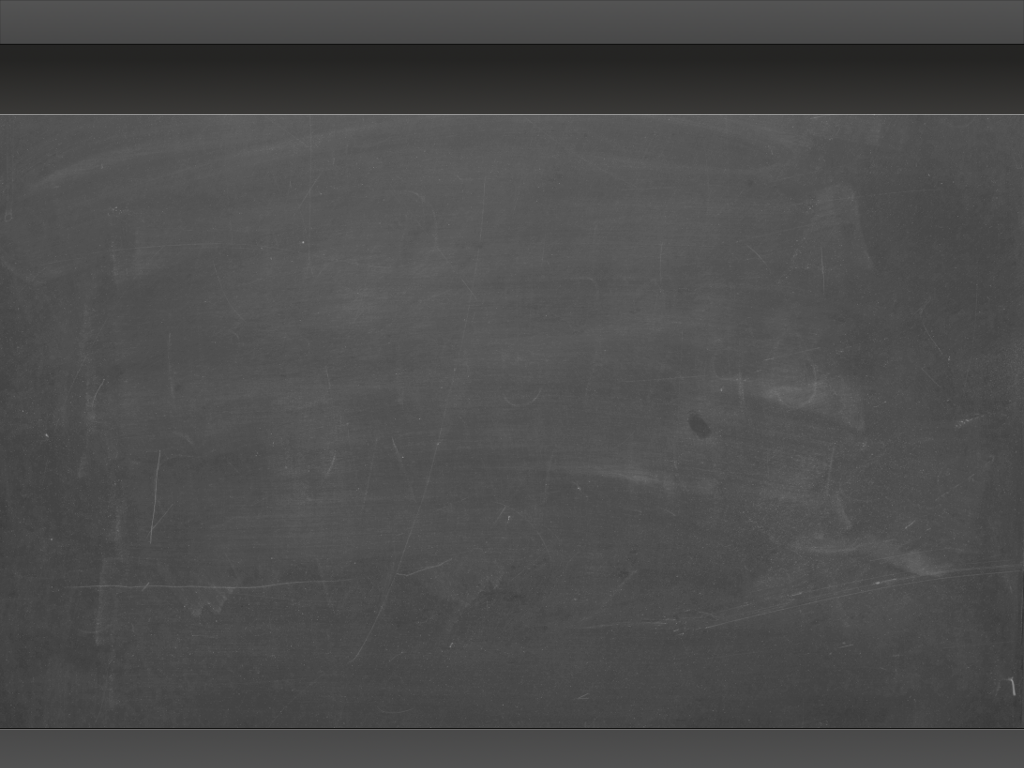
\includegraphics
	[width=\paperwidth,height=\paperheight]{background.png}}

\makeatletter
\definecolor{pbfc}{RGB}{117,137,12}% filling color for the progress bar
\definecolor{pbbg}{HTML}{282828}% background color for the progress bar
\def\progressbar@progressbar{} % the progress bar
\newcount\progressbar@tmpcounta% auxiliary counter
\newcount\progressbar@tmpcountb% auxiliary counter
\newdimen\progressbar@pbht %progressbar height
\newdimen\progressbar@pbwd %progressbar width
\newdimen\progressbar@tmpdim % auxiliary dimension

\progressbar@pbwd=70ex
\progressbar@pbht=1ex

% the progress bar
\def\progressbar@progressbar
{%
 \progressbar@tmpcounta=\insertframenumber
 \progressbar@tmpcountb=\inserttotalframenumber
 \progressbar@tmpdim=\progressbar@pbwd
 \multiply\progressbar@tmpdim by \progressbar@tmpcounta
 \divide\progressbar@tmpdim by \progressbar@tmpcountb

 \begin{tikzpicture}[rounded corners=1pt,very thin]
  % Colors
  \colorlet{border}{black}
  \shade[top color=pbbg!100,bottom color=pbbg!80,top color=pbbg!100]
   (0pt, 0pt) rectangle ++ (\progressbar@pbwd, \progressbar@pbht);
  \shade[draw=pbfc,top color=pbfc!50,bottom color=pbfc!50,middle color=pbfc] %
   (0pt, 0pt) rectangle ++ (\progressbar@tmpdim, \progressbar@pbht);
  \draw[color=border]
   (0pt, 0pt) rectangle (\progressbar@pbwd, \progressbar@pbht);
 \end{tikzpicture}%
}


\setbeamertemplate{navigation symbols}{}
\setbeamercolor{normal text}{fg=white}

\addtobeamertemplate{frametitle}{\vskip-0.25ex}{}
\addtobeamertemplate{footline}{\vskip-0.5ex}{}

\addtobeamertemplate{footline}{}
{%
 \begin{beamercolorbox}[ht=3ex,leftskip=1.5ex,rightskip=1ex]{author in head/foot}
  \progressbar@progressbar  \hspace{1.5ex} \textcolor{title}\insertframenumber
   \vspace{1.5ex}
  \end{beamercolorbox}
}
\makeatother



%%%%%%%%%%%%%%%%%%%%%%%%%%%%%%%%%%%%%%%%%%%%%%%%%%%%%%%%%%%%%%%%%%%%%%%%%%%%%%%%%%%%%%%%%%%%%%%%%%%%%%%%%%%%%%%%%%%%%%%%%%%%%%%%%%%%%%%%%%%%%%%%
%%%%%%%%%%%%%%%%%%%%%%%%%%%%%%%%%%%%%%%%%%%%%%%%%%%%%%%%%%%%%%%%%%%%%%%%%%%%%%%%%%%%%%%%%%%%%%%%%%%%%%%%%%%%%%%%%%%%%%%%%%%%%%%%%%%%%%%%%%%%%%%%
%%%%%%%%%%%%%%%%%%%%%%%%%%%%%%%%%%%%%%%%%%%%%%%%%%%%%%%%%%%%%%%%%%%%%%%%%%%%%%%%%%%%%%%%%%%%%%%%%%%%%%%%%%%%%%%%%%%%%%%%%%%%%%%%%%%%%%%%%%%%%%%%
%
%  Begin Presentation
%



\title[DSpace]{\fontsize{22}{24}\selectfont DSpace}
\subtitle[A new way of handling geolocation based information ]{\fontsize{12}{14}\selectfont \textcolor{subtitle}{A new way of handling geolocation based information }}
\author[iggy \& chrono]{\\[3ex]iggy \& chrono}

\institute[Apollo-NG]{
 
\includegraphics[scale=0.5]{apollo-mission-badge.pdf}}
}
\date[June 2013]{June 13, 2013}


\begin{document}


%--- the titlepage frame -------------------------%
{
\setbeamertemplate{background canvas}{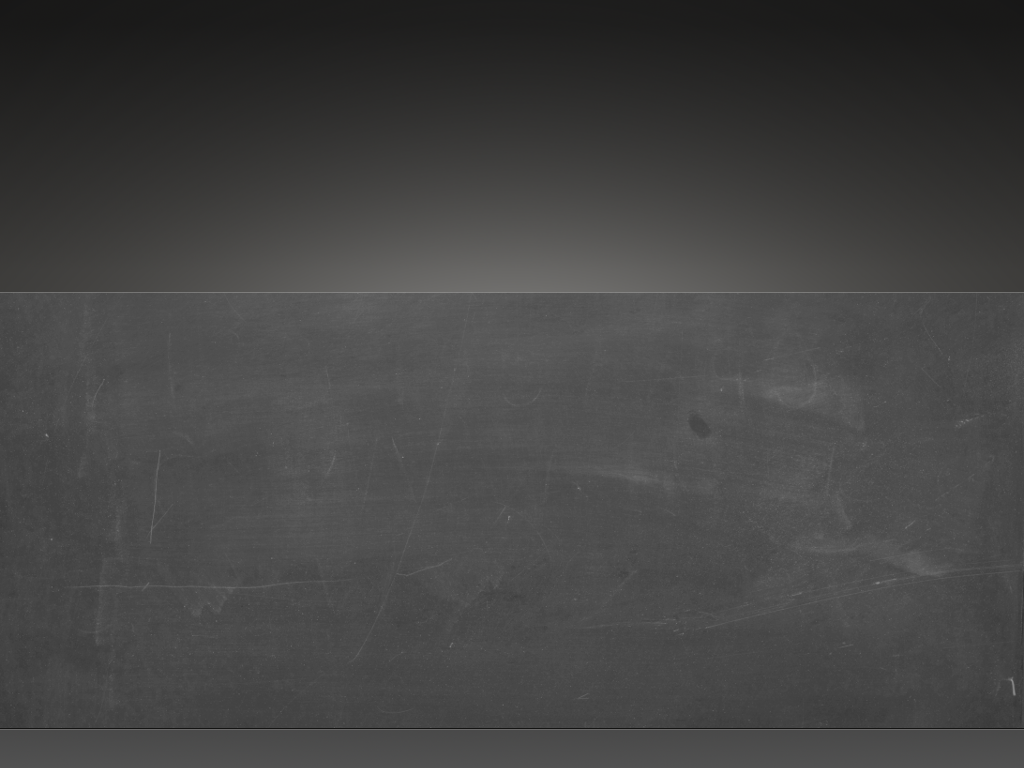
\includegraphics
 [width=\paperwidth,height=\paperheight]{background-title.png}}
\setbeamertemplate{headline}{}
\setbeamertemplate{footline}{}
\begin{frame}[plain]
 \vspace{1em}
 \titlepage
\end{frame}
}

\addtocounter{framenumber}{-1}

%--- the toc frame -------------------------%

{
\setbeamertemplate{headline}{}
\setbeamertemplate{footline}{}
\begin{frame}[plain]
\frametitle{\vspace{-2.12ex}Talk-Contents}
 \tableofcontents
\end{frame}
}

\addtocounter{framenumber}{-1}
\setcounter{page}{1}

%
%  Begin Content
%

\section{What do we want?}

\begin{frame}{Question}
 \textit{If life were a just computer game with awesome sensory input,\linebreak
  which standard game features would be missing in our interface\linebreak
  in order to play it well, especially when playing in groups?}
 \vspace{2em}
 \pause
 \begin{itemize}[<+->]
  \item A MiniMap
  \item Instant group communication
 \end{itemize}
\end{frame}

\begin{frame}{Basemaps}
 screenshot and explanation for basemaps
\end{frame}

\begin{frame}{Overlays}
 screenshot and explanation for overlays
\end{frame}

\begin{frame}{Basic rules}{with a subtitle}
 Increase the likelyhood and efficiency of adding/sharing information by introducing
 a standardized framework like the W3c in 1993.
 \begin{itemize}
  \item Federation
  \item Free to use
  \item Open Source
  \item Lose Bindings
  \item Modular Extensions
 \end{itemize}
\end{frame}

\begin{frame}{Overlay ideas}{}
 \begin{itemize}
  \item Urban Management
   \begin{itemize}
    \item Emergency Response Management (First Responder Setup)
    \item Hitchhiking (linking drivers/hikers in a sector - hitchwiki.org)
    \item Real-Time public transportation information
    \item Real-Time risk distribution
   \end{itemize}
  \item Resource Management
   \begin{itemize}
    \item Food Mapping/Sharing (mundraub/foodshare.org)
    \item Dumpster Diving (trashwiki.org)
    \item Fleet Management
    \item Open Access Mapping (openwifimap.net)
   \end{itemize}
  \item Organizing Events
   \begin{itemize}
    \item Public congress/camp Overlay for visitors
    \item Private engel Overlays for orga
   \end{itemize}

 \end{itemize}
\end{frame}

\begin{frame}{Even more Overlay ideas}{}
 \vspace{1em}
 \begin{itemize}
  \item Realtime Semantic Mapping ⇒ Heat mapping twitter hashtags (i.e. heatmap \#earthquake to find current EQ reports and positions)
  \item Private group overlays for the area of activity (i.e. MuCCC)
  \item Drone GCS Interfacing ⇒ Localization and interactive Mission/WayPoint Management
  \item Entertainment ⇒ Geocaching, AR-MMORPGs, AR-MMO-Strategy-Games
  \item Open Network Access ⇒ Mapping Access Points (http://openwifimap.net)-http://map.pberg.freifunk.net/ + ham-radio repeater information
  \item ADS-B Airplane Mapping Overlay
  \item Use your imagination
 \end{itemize}
\end{frame}





\section{What do we have?}

\begin{frame}{What do we have?}
Before we start to re-invent the wheel, let's have a look at what other
generous people already have developed and shared with the rest of humankind.
\end{frame}


\subsection{Basemaps}

\begin{frame}{Basemaps}
 \begin{columns}
  \column{.5\textwidth}
   OSM Rendered Map
  \column{.5\textwidth}
   \pause
   DSpace self-rendered Map
 \end{columns}
\end{frame}


\setbeamertemplate{blocks}[rounded]
\setbeamercolor{block body}{bg=block}
\begin{frame}[fragile]{Map Forge}
 \begin{itemize}
  \item NodeJS
  \item Mapnik + TileMill + OSM-Bright
  \item PostgreSQL + PostGIS + imposm
  \item OpenStreepMap data
  \item NASA/CGIAR SRTM SIR-C-Band V41 90m Topo data
  \item DLR SRTM X-Band SAR 25m Topo data
  \item TerraSAR-X/TanDEM-X data (Future)
 \end{itemize}
\Fontvi
\lstset{language=C++,
				numbers=left,
				numberstyle=\tiny,
				numbersep=-1.8ex,
                basicstyle=\color{black}\ttfamily,
                keywordstyle=\color{blue}\ttfamily,
                stringstyle=\color{red}\ttfamily,
                commentstyle=\color{green}\ttfamily,
                morecomment=[l][\color{magenta}]{\#}
}
\begin{block}{}
\begin{lstlisting}
    imposm -U gisuser -d gis -m \
    /tmp/osm-bright/imposm-mapping.py --overwrite-cache --read --write --optimize \
    --deploy-production-tables planet-latest.osm.pbf
\end{lstlisting}
\end{block}
\end{frame}

\begin{frame}{Map Forge Screenshot}
Include picture of Map Forge in action
\end{frame}

\begin{frame}{Map Delivery}
 \begin{itemize}
  \item NodeJS + TileStream
 \end{itemize}
\end{frame}

\begin{frame}{Map Delivery}
Live DEMO
\end{frame}

\subsection{Overlays}

\begin{frame}{Read-Only}
 \begin{itemize}
  \item Simple HTTP GeoJSON Feed
  \item SpaceAPI
 \end{itemize}
\end{frame}


\begin{frame}{Read-Write}
 \begin{itemize}
  \item remotestorage.io
 \end{itemize}
\end{frame}


\subsection{Navigation}

\begin{frame}{Navigation}
 \begin{itemize}
  \item Routino
  \item OpenStreetmap import
 \end{itemize}
\end{frame}

\begin{frame}{Read-Write}
\begin{itemize}
  \item remotestorage.io
\end{itemize}
\end{frame}


\subsection{DSpace Client}

\begin{frame}{DSpace Client}
 Introduction on the Client
\end{frame}

\begin{frame}{Javascript Dependencies}{}
 \begin{itemize}
  \item Ender
  \item Underscore
  \item Backbone
  \item Bean
  \item Bonzo
  \item DOMReady
  \item RequireJS
  \item Qwery
  \item Morpheus
  \item Reqwest
 \end{itemize}
\end{frame}

\begin{frame}{Build Dependencies}{}
 \begin{itemize}
  \item Almond (AMD)
  \item Handlebars
  \item CSSO
 \end{itemize}
\end{frame}



\section{What do we need?}

\begin{frame}{DSpace Client}
 Introduction on the Client
\end{frame}



\end{document}
